\chapter{Linear Instabilities}
\label{c_lin_inst}

\section{Drift Waves}
\label{s_drift_waves}

\begin{figure}[!htbp]
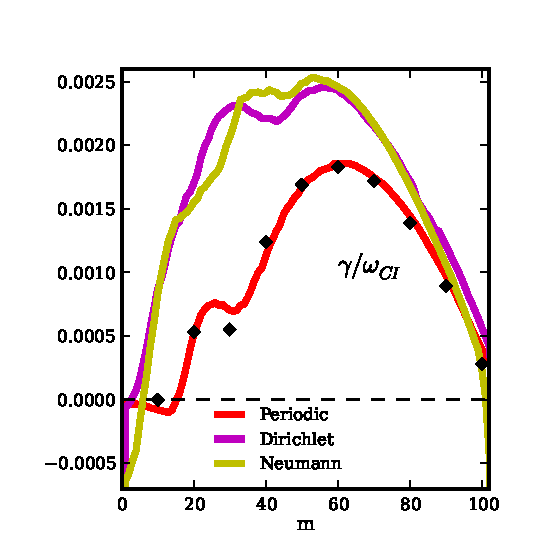
\includegraphics[]{lin_dw_gamma}
\hfil
\caption{Linear drift wave growth rates}
\label{lin_dw_gamma}
\end{figure}

\section{Conducting Wall Mode}
\label{s_cwm}

\begin{figure}[!htbp]
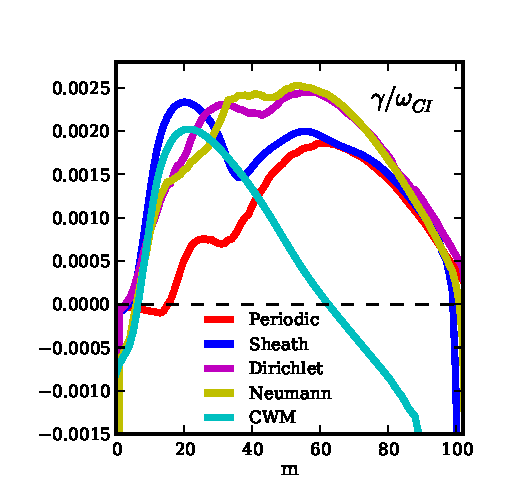
\includegraphics[]{gamma_comparisons}
\hfil
\caption{Linear conducting wall mode growth rates}
\label{gamma_comparisons}
\end{figure}


In this section, we consider the linear instability caused by a plasma bounded by two conducting walls on the boundaries where the magnetic field lines terminate (the axial boundaries).
The instability is dependent upon Bohm sheath boundary conditions that were derived in Sec.~\ref{ss_bs_bc}. As already noted, these boundary conditions are not necessarily the correct ones
for LAPD, but are somewhat idealized. Yet, it is still academically instructive to apply such an idealized boundary condition to LAPD because it creates a new linear instability, which
can be used to test the robustness of LAPD's nonlinear instability.


The conducting wall mode instability in the case considered here is purely an electron temperature gradient instability, although other types of gradients can cause it~\cite{berk1993}.
Electron temperature fluctuations are advected by electrostatic potential fluctuations and feed off the equilibrium electron temperature gradient as in the case of the thermal drift waves.
However, in contrast to the thermal drift waves, the coupling between the temperature and potential fluctuations comes through the sheath boundary condition rather than through the adiabatic
response.
